\documentclass[11pt]{article}


\usepackage[left=1in, right=1in, top=1in, bottom=1in]{geometry}
\usepackage{amsmath}
\usepackage{amsfonts}
\usepackage{graphicx}
\usepackage{listings}
\usepackage{color}
\usepackage{float}
\usepackage{caption}
\usepackage{subcaption}
\usepackage{fancyhdr}
\usepackage{pgfplots}
\usepackage{algorithm}
\usepackage{algpseudocode}
\usepackage{placeins}
\usepackage{tikz}
\usetikzlibrary{arrows.meta, positioning, calc}
\pgfplotsset{compat=1.18}

\title{Blocked Dynamic Sparse Attention}
\author{Mehul Goel (mehulg), Saransh Agrawal (saransh2) \\ \small Website: https://mehulgoel873.github.io/15418-final-project/}
\date{}

\thispagestyle{plain}
\pagestyle{fancy}
\fancyhf{}
\lhead{Blocked Dynamic Sparse Attention}
\rhead{Mehul Goel, Saransh Agrawal}
\setlength{\headheight}{14pt}

\begin{document}
\maketitle


\section*{Summary}
\section*{Background}
\subsection*{Attention}

\begin{figure}[H]
    \centering
    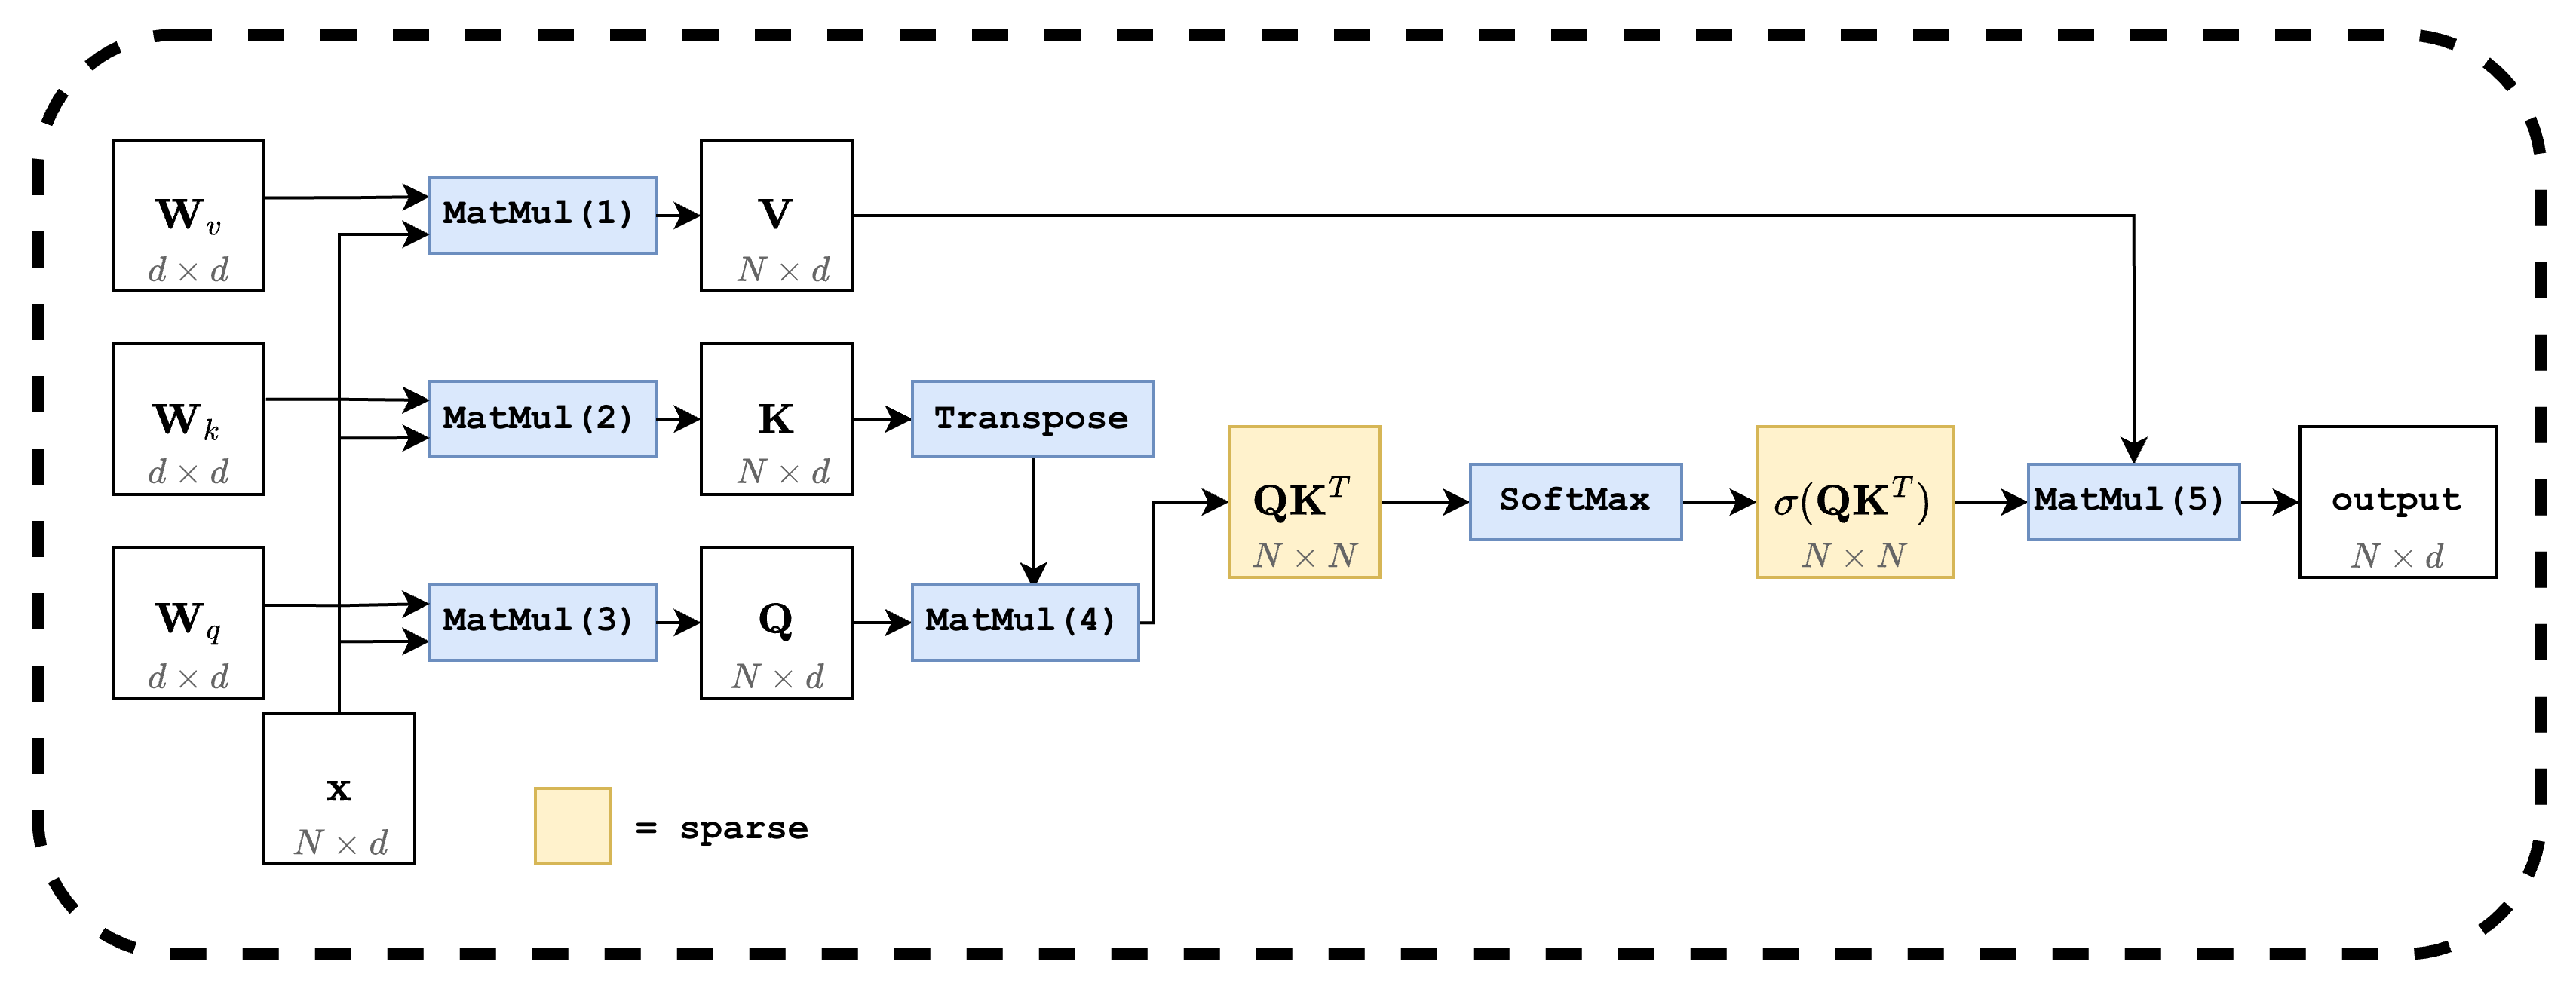
\includegraphics[width=\linewidth]{figs/attention.png}
    \caption{The attention block. Three projections (MatMuls~(1)--(3)) produce $Q$, $K$, $V$; MatMul~(4) and the softmax operate on an $N \times N$ matrix (highlighted), and MatMul~(5) collapses back to $N \times d$.}
    \label{fig:attention}
\end{figure}

Modern transformers process a sequence of tokens by repeatedly applying an \textit{attention} operation. Each token is represented as a $d$-dimensional embedding vector, so the input to an attention layer is a matrix $\mathbf{x} \in \mathbb{R}^{N \times d}$, where $N$ is the number of tokens (the \textit{context length}) and $d$ is the embedding dimension.

Figure~\ref{fig:attention} sketches the full attention block. The input $\mathbf{x}$ is first projected by three learned $d \times d$ weight matrices $\mathbf{W}_q, \mathbf{W}_k, \mathbf{W}_v$ (MatMuls~(1)--(3)) into a query $Q$, a key $K$, and a value $V$, each of shape $N \times d$. The layer then computes
\[
\text{Attention}(Q, K, V) = \text{softmax}\!\left(\frac{QK^T}{\sqrt{d}}\right) V.
\]
MatMul~(4) forms the $N \times N$ score matrix $QK^T$, a row-wise softmax turns these scores into normalized weights, and MatMul~(5) multiplies them by $V$.


The two highlighted stages in Figure~\ref{fig:attention} scale with the \emph{square} of the sequence length. MatMul~(4) materializes an $N \times N$ matrix, the softmax sweeps over it row by row, and MatMul~(5) reads it again. In practical settings $N \gg d$. Today's frontier models target context lengths of a million tokens or more, while $d$ is typically only 64 or 128 per head, so a single attention layer would touch on the order of $10^{12}$ entries in its intermediate matrix. Both the arithmetic and the memory traffic of storing and revisiting an $N \times N$ matrix become impractical at this scale.

Each block in the figure maps well to a GPU on its own. The matrix multiplications are embarrassingly parallel: each output entry can be computed independently. The softmax requires a reduction along each row, but the rows themselves are independent and parallelize across $N$. The bottleneck is therefore not a lack of parallelism but the volume of computation and data movement on an $N \times N$ matrix at long context lengths. Most entries of the softmax output are close to zero (highlighted as ``sparse'' in Figure~\ref{fig:attention}), and that observation motivates the tiled and sparse approaches we explore in the rest of this report.


\subsection*{Sparsity}

A long line of work has shown that the score matrix $\sigma(QK^T)$ produced by attention is approximately sparse: most of its entries are very small after the row-wise softmax, and the output of MatMul~(5) is dominated by a small fraction of the columns. This has motivated a broad family of \emph{sparse attention} schemes that fall into two camps. Static patterns (such as local windows, strided, or block-diagonal masks) fix a sparsity structure ahead of time and are easy to map onto regular GPU tile layouts. Dynamic patterns (such as top-$k$ or learned routing) choose which entries to keep based on the input itself, often giving better accuracy at a given sparsity level at the cost of more irregular computation~\cite{lin2021survey}.

Rather than commit to a single pattern, our experiments use a randomly-generated sparse mask. Each cell is independently kept with probability $p$, where $p$ is the fraction of dense entries. This lets us sweep sparsity levels without entangling our results with the biases of any particular method. To match the granularity at which real-world transformers exploit sparsity, the mask is defined at a \emph{block} level rather than per-element: a granularity of $g$ means we partition the $N \times N$ score matrix into $g \times g$ tiles and label each tile as fully dense or fully sparse. A granularity of $1$ corresponds to per-element sparsity, while a granularity of $32$ means $32 \times 32$ tiles are the smallest unit of sparsity.

Block-level sparsity reduces the total amount of work on the score matrix, but it gives up structure that dense kernels rely on. Coalesced memory accesses, vectorized loads, and predictable load balancing all assume regular tile traversal; once tiles are skipped according to a mask, warps within a thread block can be assigned very different amounts of work, the rows of the score matrix lose alignment in memory, and arithmetic intensity drops. Recovering performance therefore requires both a sparse-friendly storage format and kernels that revisit the three stages of attention with the mask in mind.

\paragraph{BCSR storage.}
We store the block-level mask in \emph{Blocked Compressed Sparse Row} (BCSR) format. BCSR is the block analogue of \emph{Compressed Sparse Row} (CSR), a standard sparse-matrix layout that stores only the nonzero values along with the column index of each one and a per-row offset into that list. BCSR does the same thing at the granularity of fixed-size tiles: instead of recording the position of every individual nonzero, it records the position of every nonzero \emph{tile}. For each row of tiles, we store the column indices of the dense tiles, and the dense tiles themselves are laid out contiguously in memory in row-major order. This keeps the inner loop of every kernel operating on dense, contiguous tiles (so coalescing and vectorization still apply within a tile) while cutting work in proportion to the fraction of sparse tiles.

\paragraph{Sparsity in MatMul.}
The two matrix multiplications in Figure~\ref{fig:attention} change shape under block sparsity. MatMul~(4) computes $QK^T$, but only at positions where the mask is dense. This is the \emph{sampled dense-dense matrix multiplication} (SDDMM) pattern: $Q$ and $K$ are dense, and the mask selects which output tiles to compute. Skipping a sparse output tile skips an entire block of dot-product reductions, which is where most of the savings come from. MatMul~(5) computes $\sigma(QK^T) \cdot V$, where the left operand is now a block-sparse matrix in BCSR form and $V$ is dense. This is the \emph{sparse-dense matrix multiplication} (SpMM) pattern: each dense tile of the score matrix contributes a small dense matmul with the corresponding rows of $V$, and the BCSR row indexing tells each thread block which tiles to accumulate.

\paragraph{Sparsity in Softmax.}
The row-wise softmax sits between MatMul~(4) and MatMul~(5), and it has to respect the same mask. Sparse tiles can be treated as containing $-\infty$ scores, so they contribute zero to both the per-row sum and the output. We never materialize those tiles in practice: the softmax kernel walks the BCSR row directly, computes the per-row max and the exponential sum across only the dense tiles in that row, and writes back the normalized values in place. The reduction structure is the same as in dense softmax, but the length of each reduction is now proportional to the number of dense tiles in the row rather than to $N$.

\paragraph{Workload characterization.}
At moderate granularities, all three sparse stages stay data-parallel at the tile level. SDDMM (MatMul~(4)) and SpMM (MatMul~(5)) decompose into independent per-tile dense matrix multiplications with no cross-tile dependencies, while the sparse softmax does a per-row reduction (max and exponential sum) over only the dense tiles in a row, and the rows themselves remain independent. Locality is strong inside a tile because operands are dense and contiguous in memory, and BCSR's row-stationary layout keeps each row's column indices and dense values close together, so a kernel sweeping a row sees a tight access pattern. SIMD execution is effective on the inner $g \times g$ matmul, where each warp runs a regular dense kernel.

This picture degrades sharply at small granularities ($g \in \{1, 2, 4\}$). At $g=1$ the workload is essentially a scatter-gather, and even at $g=2$ or $4$ each tile is smaller than a warp, so the inner dense matmul cannot fill 32 SIMT lanes and tensor-core or vector instructions cannot reach their minimum operand sizes. A single warp ends up assigned to multiple adjacent tiles whose mask bits diverge, forcing serialized execution within the warp. BCSR's per-tile metadata (a column-index lookup and a row-pointer dereference) also becomes comparable in cost to the actual compute, so memory traffic is dominated by indexing rather than values. Even at larger granularities the scheduling unit is now a variable-length list of dense tiles rather than a fixed row of $N$ elements, so load imbalance across thread blocks is the primary cost we have to contain.


\section*{Approach}
\subsection*{Tiled Matmul}
Before diving into the three different kernels, it's best to start with a brief explanation of our baseline: Tiled Matrix Multiplication. In tiled matmul, we are multiplying two matrices, $A \in \mathbb{R}^{M \times K}, B \in \mathbb{R}^{K \times N}$, $A \cdot B = C$. To do this on an NVIDIA GPU, we utilize CUDA kernilization, targetting a Blackwell RTX 6000. 

If you mapped each thread independently to a singular thread within a thread block, the code would be: $C_{ij} = \sum_{k = 0}^{K} A_{ik} \cdot B_{kj}$, launched for $M \cdot N$ threads. However, there is an opportunity for data reuse, a thread at location $C_{i, j}$, and a thread for $C_{i + 1, j}$ will both independently reload $A_i$. Thus we can utilize the shared memory on a thread block within CUDA cores (around 128 KB of L1 cache for Blackwell 6000), mapping each thread block to a $T \times T$ tile of $C$, where we load $a = A_{(i:i+T, k)}, b = B_{(k, j:j+t)} \forall k$. Then $C_{(i:i+T, j:j+T)} = ab$, and each element can be mapped to an individual thread. 
% Insert Tiled Matmul BRIEF Pseudcode

\subsection*{Sparse Matrix Multiplication (SpMM)}


\section*{Results}

\bibliographystyle{plain}
\bibliography{references}



\section*{List of work}
The total credit for the project was 50-50 between Saransh and Mehul. 



\end{document}
